\documentclass{article}

% preamble
\def\npart{III}
\def\nyear{2019}
\def\nterm{Lent}
\def\draft{Ongoing course}
\def\nlecturer{Professor B. L\"owe}
\def\ncourse{Topics in Set Theory}

\usepackage{imakeidx}
\usepackage{mathrsfs}
\usepackage{marginnote}
\usepackage{pbox}

\ifx \nauthor\undefined
  \def\nauthor{Bhavik Mehta}
\else
\fi

\author{Based on lectures by \nlecturer \\\small Notes taken by \nauthor}
\date{\nterm\ \nyear}
\title{Part \npart\ -- \ncourse}

\usepackage[utf8]{inputenc}
\usepackage{amsmath}
\usepackage{amsthm}
\usepackage{amssymb}
\usepackage{enumerate}
\usepackage{mathtools}
\usepackage{graphicx}
\usepackage[dvipsnames]{xcolor}
\usepackage{tikz}
\usepackage{wrapfig}
\usepackage{centernot}
\usepackage{float}
\usepackage{braket}
\usepackage[hypcap=true]{caption}
\usepackage{enumitem}
\usepackage[colorlinks=true, linkcolor=mblue]{hyperref}
\usepackage[nameinlink,noabbrev]{cleveref}
\usepackage{nameref}
\usepackage[margin=1.5in]{geometry}

% Theorems
\theoremstyle{definition}
\newtheorem*{aim}{Aim}
\newtheorem*{axiom}{Axiom}
\newtheorem*{claim}{Claim}
\newtheorem*{cor}{Corollary}
\newtheorem*{conjecture}{Conjecture}
\newtheorem*{defi}{Definition}
\newtheorem*{eg}{Example}
\newtheorem*{ex}{Exercise}
\newtheorem*{fact}{Fact}
\newtheorem*{law}{Law}
\newtheorem*{lemma}{Lemma}
\newtheorem*{notation}{Notation}
\newtheorem*{prop}{Proposition}
\newtheorem*{question}{Question}
\newtheorem*{rrule}{Rule}
\newtheorem*{thm}{Theorem}
\newtheorem*{assumption}{Assumption}

\newtheorem*{remark}{Remark}
\newtheorem*{warning}{Warning}
\newtheorem*{exercise}{Exercise}

% \newcommand{\nthmautorefname}{Theorem}

\newtheorem{nthm}{Theorem}[section]
\newtheorem{nlemma}[nthm]{Lemma}
\newtheorem{nprop}[nthm]{Proposition}
\newtheorem{ncor}[nthm]{Corollary}
\newtheorem{ndef}[nthm]{Definition}

% Special sets
\newcommand{\C}{\mathbb{C}}
\newcommand{\N}{\mathbb{N}}
\newcommand{\Q}{\mathbb{Q}}
\newcommand{\R}{\mathbb{R}}
\newcommand{\Z}{\mathbb{Z}}

\newcommand{\abs}[1]{\left\lvert #1\right\rvert}
\newcommand{\norm}[1]{\left\lVert #1\right\rVert}
\renewcommand{\vec}[1]{\boldsymbol{\mathbf{#1}}}

\let\Im\relax
\let\Re\relax

\DeclareMathOperator{\Im}{Im}
\DeclareMathOperator{\Re}{Re}
\DeclareMathOperator{\id}{id}

\definecolor{mblue}{rgb}{0., 0.05, 0.6}

\swapnumbers

\makeindex[intoc]

\renewcommand{\arraystretch}{1.3}

\newcommand{\named}[1]{\textbf{#1}\index{#1}}
\newcommand{\bonusnamed}[1]{\textbf{#1}\index{#1@*#1}}
\DeclareMathOperator{\dom}{dom}
\DeclareMathOperator{\ran}{ran}
\DeclareMathOperator{\rk}{rk}
\DeclareMathOperator{\cons}{Cons}
\DeclareMathOperator{\tcl}{tcl}

\setcounter{section}{-1}

\let\oldmodels\models
\let\models\vDash
\let\nModels\nvDash

\tikzset{dot/.style={inner sep=1pt, fill=black, circle}}

% and here we go!
\begin{document}
\maketitle

\tableofcontents

\clearpage
\section{Introduction}
\newlec
The main `topic in set theory' covered in this course will be one of the most important: solving the Continuum Problem.
A priori, set theory does not seem intrinsically related to logic, but the continuum hypothesis showed that logic was a very important tool in set theory.
In contrast to many other disciplines of mathematics, in set theory we typically try to prove things are \emph{impossible}, rather than showing what is possible.

The second international congress of mathematicians in 1900 was in Paris, where Hilbert spoke. At that time, Hilbert was a `universal' mathematician, and had worked in every major field of mathematics. He gave a list of problems for the century, the 23 Hilbert Problems. The first on this list was the Continuum Problem.

\subsection{Continuum Hypothesis}\index{Continuum hypothesis}\hypertarget{def:ch}
Here is Hilbert's formulation of the Continuum hypothesis (CH):
Every set of infinitely many real numbers is either equinumerous with the set of natural numbers or the set of real numbers.
More formally, we might write
\begin{equation*}
  \forall X \subseteq \mathbb{R}, (X \text{ is infinite} \Rightarrow X \sim \mathbb{N} \text{ or } X \sim \mathbb{R})
\end{equation*}

In more modern terms, we write this as the claim $2^{\aleph_0} = \aleph_1$.
These two statements are equivalent (in \textsf{ZFC}).

Assume that $2^{\aleph_0} > \aleph_1$, in particular $2^{\aleph_0} \geq \aleph_2$. Since $2^{\aleph_0} \sim \mathbb{R}$, we get an injection $i: \aleph_2 \to \mathbb{R}$.
Consider $X \coloneqq i[\aleph_1] \subseteq \mathbb{R}$. Clearly, $i|_{\aleph_1}$ is a bijection between $\aleph_1$ and $X$, so $X \sim \aleph_1$.
But $\aleph_1 \nsim \mathbb{N}$ and $\aleph_1 \nsim \mathbb{R}$.
Thus $X$ refutes CH (in its earlier formulation).
So: $2^{\aleph_0} \neq \aleph_1 \implies \neg \text{CH}$.

If $2^{\aleph_0} = \aleph_1$.
Let $X \subseteq \mathbb{R}$. Consider $b: 2^{\aleph_0} \to \mathbb{R}$ a bijection. If $X$ is infinite, then $b^{-1}[X] \subseteq 2^{\aleph_0}$.
Thus the cardinality of $X$ is either $\aleph_0$, i.e.\ $X \sim \mathbb{N}$ or $\aleph_1$, i.e.\ $X \sim \mathbb{R}$.
So, $2^{\aleph_0} = \aleph_1 \implies \text{CH}$.

\subsection{History of CH}
\begin{itemize}[label=--]
  \item 1938, G\"odel: \textsf{ZFC} does not prove $\neg$\hyperlink{def:ch}{CH}.
  \item 1963, Cohen: \textsf{ZFC} does not prove CH.
\end{itemize}
G\"odel's proof used the technique of inner models; Cohen's proof used forcing, sometimes referred to as outer models.

G\"odel's Completeness Theorem:
\begin{equation*}
  \text{Cons}(T) \iff \exists(M, E) (M, E) \models T
\end{equation*}
From this, we might guess that G\"odel's and Cohen's proof will show there is a model of \textsf{ZFC} + CH, and a model of \textsf{ZFC} + $\neg$CH, but by the incompleteness phenomenon, we cannot prove there is a model of \textsf{ZFC}!
So, we are not going to be able to prove Cons(\textsf{ZFC}+CH), but instead
\begin{equation*}
  \text{Cons(\textsf{ZFC})} \rightarrow \text{Cons(\textsf{ZFC}+CH)}
\end{equation*}
Or, equivalently,
\begin{equation*}
  \text{if } M \models \text{\textsf{ZFC}, then there is } N \models \text{\textsf{ZFC} + CH}.
\end{equation*}

\clearpage
\section{Model theory of set theory}
Let's assume for a moment that
\begin{equation*}
  (M,\in) \models \text{\textsf{ZFC}}.
\end{equation*}
We refer to the canonical objects in $M$ by the usual symbols, e.g., $0,1,2,3,4,\dotsc, \omega, \omega+1, \dotsc$

What would an ``inner model'' be?
Take $A \subseteq M$, and consider $(A, \in)$. This is a substructure of $(M, \in)$.
Note: the language of set theory has no function or constant symbols. But we write down
\begin{equation*}
  X = \emptyset,\ X = \{Y\},\ X = \{Y,Z\},\ X = \bigcup Z,\ X = \mathcal{P}(Z)
\end{equation*}
which appear to use function or constant symbols. These are technically not part of the language of set theory; they are abbreviations:
\begin{align*}
  X &= \emptyset & &\text{ abbreviates } & &\forall w\; (\neg w \in X) \\
  X &= \{Y\} & & \text{ abbreviates } & &\forall w\; (w \in X \leftrightarrow w = Y) \\
  X &\subseteq Y & & \text{ abbreviates } & &\forall w\; (w \in X \rightarrow w \in Y)
\end{align*}
and so on.

\begin{defi}\hypertarget{def:abso}
  If $\varphi$ is a formula in $n$ free variables. We say
  \begin{enumerate}[label=(\arabic*)]
    \item $\varphi$ is \named{upwards absolute}\index{absolute!upwards-} between $A$ and $M$ if
      \begin{equation*}
        \text{for all } a_1, \dotsc, a_n \in A,\quad (A,\in) \models \varphi(a_1, \dotsc, a_n) \implies (M, \in) \models \varphi(a_1, \dotsc, a_n)
      \end{equation*}
    \item $\varphi$ is \named{downwards absolute}\index{absolute!downwards-} between $A$ and $M$ if
      \begin{equation*}
        \text{for all } a_1, \dotsc, a_n \in A,\quad (M,\in) \models \varphi(a_1, \dotsc, a_n) \implies (A, \in) \models \varphi(a_1, \dotsc, a_n)
      \end{equation*}
    \item $\varphi$ is \named{absolute} between $A$ and $M$ if it is upwards absolute and downwards absolute.
  \end{enumerate}
\end{defi}

\begin{defi}
  We\index{quantifier-free} say that a formula is \hypertarget{def:sig1}$\Sigma_1$ if it is of the form
  \begin{equation*}
    \exists x_1 \dotsc \exists x_n\ \varphi(x_1, \dotsc, x_n) \text{ where } \varphi \text{ is quantifier-free}
  \end{equation*}
  or \hypertarget{def:pi1}{$\Pi_1$} if it is of the form
  \begin{equation*}
    \forall x_1 \dotsc \forall x_n\ \varphi(x_1, \dotsc, x_n) \text{ where } \varphi \text{ is quantifier-free}.
  \end{equation*}
\end{defi}

\begin{remark}
  \leavevmode
  \begin{enumerate}[label=(\alph*)]
    \item If $\varphi$ is quantifier-free, then $\varphi$ is \hyperlink{def:abso}{absolute} between $A$ and $M$.
    \item If $\varphi$ is \hyperlink{def:pi1}{$\Pi_1$}, then it's \hyperlink{def:abso}{downward absolute}
    \item If $\varphi$ is \hyperlink{def:sig1}{$\Sigma_1$}, then it's \hyperlink{def:abso}{upward absolute}
  \end{enumerate}
\end{remark}

\newlec
Under our assumption that $(M,\in) \models \text{\textsf{ZFC}}$, which subsets $A \subseteq M$ give a model of \textsf{ZFC}?
Using standard model theory, we observed that if $\varphi$ is quantifier-free, then $\varphi$ is \hyperlink{def:abso}{absolute} between $(A,\in)$ and $(M,\in)$, but hardly anything is quantifier-free:
\begin{equation*}
  \hypertarget{def:phi0}x = \emptyset \iff \forall w\ (w \notin x) \eqqcolon \Phi_0(x)
\end{equation*}

For instance, suppose $A \coloneqq M \setminus \{1\}$ (recall $0,1,2,\dotsc$ refer to the ordinals in $M$).
In $A$, we have $0,2,\{1\}$. Clearly $(M,\in) \models \Phi_0(0)$.
$\Phi_0(x)$ is a \hyperlink{def:pi1}{$\Pi_1$} formula, so by $\Pi_1$-\hyperlink{def:abso}{downwards absoluteness}, $(A,\in) \models \Phi_0(0)$.

In reality, $2 = \{0,1\}$, but $1$ is not in $A$, so informally in $A$, the object $2$ has only one element.
Similarly, in $A$, $\{1\}$ has no elements, since $1$ is missing from $A$. Thus
\begin{equation*}
  (A,\in) \models \Phi_0(\{1\}).
\end{equation*}
Clearly $(M,\in) \nModels \Phi_0(\{1\})$, so $\Phi_0$ is not \hyperlink{def:abso}{absolute} between $A$ and $M$.
As a corollary, we get $(A,\in) \nModels$ Extensionality, since $0$ and $\{1\}$ have the same elements in $A$, but are not equal.

(Remark: We could go on, defining formulas $\Phi_1(x), \Phi_2(x)$ etc.\ to analyse which of the elements correspond to the natural numbers in $A$.)

\begin{defi}\hypertarget{def:transitive}
  We call $A$ \named{transitive} in $M$, if for all $a \in A$ and $x \in M$ such that $(M,\in) \models x \in a$, we have $x \in A$.
\end{defi}
\begin{prop}
  If $A$ is \hyperlink{def:transitive}{transitive}, then \hyperlink{def:phi0}{$\Phi_0$} is \hyperlink{def:abso}{absolute} between $A$ and $M$.
\end{prop}
\begin{proof}
  Since \hyperlink{def:phi0}{$\Phi_0$} is \hyperlink{def:pi1}{$\Pi_1$}, we only need to show \hyperlink{def:abso}{upwards absoluteness}.
  Suppose $a \in A$, such that $(A,\in) \models \Phi_0(a)$.
  Suppose $a \neq 0$. Thus there is some $x \in a$. By \hyperlink{def:transitive}{transitivity}, $x \in A$.
  So $(A,\in) \models x \in a$ and so $(A,\in) \nModels \Phi_0(a)$, contradiction.
\end{proof}
(Similarly, if $\Phi_n$ is the formula describing the natural number $n$, and there is $a \in A$ such that $(A,\in) \models \Phi_n(a)$ and $A$ is \hyperlink{def:transitive}{transitive}, then $a = n$.)
\begin{prop}
  If $A$ is \hyperlink{def:transitive}{transitive} in $M$, then
  \begin{equation*}
    (A,\in) \models \textsf{Ext}.
  \end{equation*}
\end{prop}
\begin{proof}
  Take $a,b \in A$ with $a \neq b$.
  By Extensionality in $(M,\in)$, find without loss of generality some $c \in a \setminus b$.
  Since $c \in a \in A$, by \hyperlink{def:transitive}{transitivity}, $c \in A$.
  Thus
  \begin{align*}
    (A,\in) &\models c \in a \\
    (A,\in) &\models c \notin b,
  \end{align*}
  so $a$ and $b$ do not satisfy the assumptions of Extensionality.
\end{proof}

Consider now $A \coloneqq \omega + 2 \subseteq M$, the ordinal consisting of $\{0,1,2,\dotsc, \omega, \omega+1\}$.
This is a transitive subset of $M$ (since it's an ordinal).
So
\begin{equation*}
  (A,\in) \models \textsf{Ext}.
\end{equation*}
Consider the formula $x = \mathcal{P}(y)$, which we can informally define as $x = \{z \mid z \subseteq y\}$, but this is not good enough. More properly, we try
\begin{equation*}
  \mathcal{P}(x) = \forall w \; (w \in x \leftrightarrow w \subseteq y).
\end{equation*}
This still includes the symbol $\subseteq$, so still needs improving.
\begin{equation*}
  \mathcal{P}(x) = \forall w \; (w \in x \leftrightarrow (\forall v \; (v \in w \rightarrow v \in y)))
\end{equation*}
In $A$, what is $\mathcal{P}(0)$?
\begin{equation*}
  (A,\in) \models \omega + 1 = \mathcal{P}(\omega)
\end{equation*}

\subsection{Bounded quantification}
We define\index{bounded quantifier}
\begin{align*}
  \exists (v \in w) \; \varphi &:\Longleftrightarrow \exists v \; (v \in w \land \varphi) \\
  \forall (v \in w) \; \varphi &\vcentcolon\Longleftrightarrow \forall v \; (v \in w \rightarrow \varphi).
\end{align*}
\begin{defi}\hypertarget{def:delta0}
  A formula $\varphi$ is called $\Delta_0$ if it is in the smallest set of formulas with the following properties
  \begin{enumerate}
    \item All quantifier-free formulas are in $S$.
    \item If $\varphi, \psi \in S$ then so are
      \begin{enumerate}
        \item $\varphi \land \psi$, $\varphi \lor \psi$, $\varphi \rightarrow \psi$, $\varphi \leftrightarrow \psi$
        \item $\neg \varphi$
        \item $\exists (v \in w) \; \varphi$, $\forall (v \in w)\; \varphi$.
      \end{enumerate}
  \end{enumerate}
\end{defi}
\begin{thm}
  If $\varphi$ is \hyperlink{def:delta0}{$\Delta_0$} and $A$ is \hyperlink{def:transitive}{transitive}, then $\varphi$ is \hyperlink{def:abso}{absolute} between $A$ and $M$.
\end{thm}
\begin{proof}
  We already knew that quantifier free formulas are \hyperlink{def:abso}{absolute}.
  Absoluteness is obviously preserved under propositional connectives.
  So, let's deal with (2c):
  Let's just do
  \begin{equation*}
    \varphi \mapsto \exists (v \in w) \; \varphi = \exists v \; (v \in w \land \varphi).
  \end{equation*}
  So suppose $\varphi$ is absolute. We need to deal with \hyperlink{def:abso}{downwards absoluteness}.
  \begin{align*}
    (M,\in) &\models \exists (v \in a) \; \varphi(v,a) \quad \text{for some } a \in A \\
    (M,\in) &\models \exists v \; (v \in a \land \varphi(v,a)).
    \intertext{Let's find $m \in M$ such that }
    (M,\in) &\models m \in a \land \varphi(m,a).
  \end{align*}
  \hyperlink{def:transitive}{Transitivity} gives $m \in A$.
  By absoluteness of $\varphi$, we get
  \begin{equation*}
    (A,\in) \models m \in a \land \varphi(m,a) \implies (A,\in) \models \exists (v \in a) \; \varphi(v,a). \qedhere
  \end{equation*}
\end{proof}

\begin{defi}
  \hypertarget{def:delta0t}{\hypertarget{def:sig1t}{\hypertarget{def:pi1t}L}}et $T$ be any `set theory'.
  Then we say that $\varphi$ is $\Delta_0^T$ if there is a \hyperlink{def:delta0}{$\Delta_0$} formula $\psi$ such that $T \vdash \phi \leftrightarrow \psi$.
  \begin{itemize}
    \item $\varphi$ is called $\Sigma_1^T$ if it is $T$-equivalent to $\exists v_1 \dots \exists v_n \; \psi$ where $\psi$ is $\Delta_0$.
    \item $\varphi$ is called $\Pi_1^T$ if it is $T$-equivalent to $\forall v_1 \dots \forall v_n \; \psi$ where $\psi$ is $\Delta_0$.
  \end{itemize}
\end{defi}
\begin{cor}
  If $A$ is \hyperlink{def:transitive}{transitive} in $M$ and both $(M,\in)$ and $(A,\in)$ are models of $T$, then \hyperlink{def:delta0t}{$\Delta_0^T$} formulas are \hyperlink{def:abso}{absolute} between $A$ and $M$, and $\Sigma_1^T, (\Pi_1^T)$ formulas are upwards (downwards) absolute between $A$ and $M$.
\end{cor}
\begin{defi}\hypertarget{def:delta1t}
  \newlec
  A formula is called $\Delta_1^T$ if it is both \hyperlink{def:sig1t}{$\Sigma_1^T$} and \hyperlink{def:pi1t}{$\Pi_1^T$}.
\end{defi}
\begin{cor}
  If $A$ is \hyperlink{def:transitive}{transitive}, $A,M \models T$ and $\varphi$ is \hyperlink{def:delta1t}{$\Delta_1^T$}, then $\varphi$ is \hyperlink{def:abso}{absolute} between $A$ and $M$.
\end{cor}
\subsection{`Set theory'}
\hypertarget{def:axioms}What do we mean by a `set theory'? The usual theories we care about are:

\begin{center}
\begin{tabular}{|rl|rl|}\hline
  \color{mred}{\textsf{FST}$_0$} & \begin{tabular}{@{}l@{}} Extensionality \\ Pairing \\ Union \\ \vspace{1mm} PowerSet \\ \vspace{1mm}\pbox{5cm}{Separation\\ (Aussonderung)} \end{tabular} & \color{mred}{\textsf{FST}} & \textsf{FST}$_0$ + \pbox{5cm}{Foundation\\ (Regularity)} \\ \hline
  \color{mred}{\textsf{Z}$_0$} & \textsf{FST}$_0$ + Infinity & \color{mred}{\textsf{Z}} & \textsf{Z}$_0$ + Foundation \\ \hline
  \color{mred}{\textsf{ZF}$_0$} & \textsf{Z}$_0$ + \pbox{5cm}{\vspace{1mm}Replacement\\ \vspace{1mm}(Ersetzung)} & \color{mred}{\textsf{ZF}} & \textsf{ZF}$_0$ + Foundation \\ \hline
  \color{mred}{\textsf{ZFC}$_0$} & \textsf{ZF}$_0$ + Choice & \color{mred}{\textsf{ZFC}} & \textsf{ZFC}$_0$ + Foundation \\ \hline
\end{tabular}
\end{center}

The subscript 0 denotes the absence of Foundation.

\subsection{A long list of \texorpdfstring{$\Delta_0^T$}{Delta0T} formulas}
We noted earlier that there are very few \hyperlink{def:delta0}{$\Delta_0$} formulas, so can we find any \hyperlink{def:delta0t}{$\Delta_0^T$} formulas?
\begin{enumerate}
  \item $x \in y$ (in fact, \hyperlink{def:delta0}{$\Delta_0$})
  \item $x = y$ (in fact, $\Delta_0$)
  \item $x \subseteq y$. This is an abbreviation, so we have to define what it means:
    \begin{equation*}\forall w\ (w \in x \rightarrow w \in y).\end{equation*}
    But note this is $\forall (w \in x) \ (w \in y)$, so $\Delta_0$.
  \item
    \begin{align*}
      \Phi_0(t) &:\Longleftrightarrow\ \forall w\ (w \notin x) \\
                &\iff \forall w\ (\neg w \in x) \\
                &\iff \forall w \ (w \in x \rightarrow \neg x = x)
    \end{align*}
    so it's $\Delta_0$ in predicate logic.
\end{enumerate}
\begin{defi}\hypertarget{def:operation}
  We say that an \named{operation} $x_1, \dotsc, x_k \mapsto F(x_1, \dotsc, x_n)$ is defined by a formula in class $\Gamma$ (where $\Gamma$ is any class of formulas) in the theory $T$ if there is a formula $\Phi \in \Gamma$ such that
\end{defi}
\begin{enumerate}[(1)]
  \item $T \vdash \forall x_1 \dotsm \forall x_n \ \exists y \ \Phi (x_1, \dotsc, x_n, y)$
  \item $T \vdash \forall x_1 \dotsm \forall x_n \ \forall y,z \ \Phi(x_1, \dotsc, x_n, y) \land \Phi(x_1, \dotsc, x_n, z) \rightarrow y = z$
  \item $\Phi(x_1, \dotsc, x_n, y)$ if and only if $y = F(x_1, \dotsc, x_n)$.
\end{enumerate}
\begin{eg}
  \begin{align*}
    x &\mapsto \{x\} \\
    x,y &\mapsto \{x,y\}
  \end{align*}
  These are \hyperlink{def:operation}{operations} in \hyperlink{def:axioms}{\textsf{FST}$_0$}!
\end{eg}
\begin{enumerate}
  \setcounter{enumi}{4}
  \item $x \mapsto \{x\}$. The formula to express this is
    \begin{align*}
      `z = \{x\}\text{'} &\iff \Phi(x,z) \\
                  &\iff \forall w \; (w \in z \leftrightarrow w = x) \\
                  &\iff \forall w \; ((w \in z \rightarrow w = x) \land (w = x \rightarrow w \in z)) \\
                  &\iff \exists (w \in z) \; (w = w) \land \forall (w \in z) \ (w = x)
    \end{align*}
    So this is $\Delta_0$ in some weak set theory.
  \item $x,y \mapsto \{x,y\}$
  \item $x,y \mapsto x \cup y$
  \item $x,y \mapsto x \cap y$
  \item $x,y \mapsto x \setminus y$
  \item $x,y \mapsto (x,y)$, where $(x,y) = \{\{x\},\{x,y\}\}$ which is the combination of earlier formulas
\end{enumerate}
If two \hyperlink{def:operation}{operations} $f, g_1, g_2$ are defined by $\Delta_0^T$-formulas, then so is the operation
\begin{equation*}
  x_1, \dotsc, x_n \mapsto f(g_1(x_1, \dotsc, x_n), \dotsc, g_k(x_1, \dotsc, x_n))
\end{equation*}
\begin{enumerate}
  \setcounter{enumi}{10}
  \item $x \mapsto x \cup \{x\} \eqqcolon S(x)$.
    By the previous fact from 5.\ and 7.
  \item $x \mapsto \bigcup x$
  \item the formula describing `$x$ is transitive'
  \item the formula describing `$x$ is an ordered pair' (the quantifiers for the two components of $x$ are bounded by $\bigcup x$)
  \item $x,y \mapsto x \times y$
  \item the formula `$x$ is a binary relation' (again, the quantifiers can be made bounded)
  \item $x \mapsto \dom(x) \coloneqq \{y | \exists p \in x; (p\text{ is an ordered pair},\ p = (v,w),\ y=v)\}$
  \item $x \mapsto \ran(x) \coloneqq \{y | \exists p \in x; (p\text{ is an ordered pair},\ p = (v,y))\}$
  \item the formula `$x$ is a function'
  \item the formula `$x$ is injective'
  \item the formula `$x$ is function from $A$ to $B$'
  \item the formula `$x$ is a surjection from $A$ to $B$'
  \item the formula `$x$ is a bijection from $A$ to $B$'
\end{enumerate}
What is an ordinal?
\begin{defi}\hypertarget{def:ordinal}
$\alpha$ is an \named{ordinal} if $\alpha$ is a \hyperlink{def:transitive}{transitive} set well-ordered by $\in$, i.e.\ it is totally ordered (several axioms, all $\Delta_0^T$) and well-founded:
\begin{equation*}
\forall X\; (X \subseteq \alpha \rightarrow X \text{ has a} \in\text{-least element}).
\end{equation*}
\end{defi}

Observe `$(X,R)$ is a well-founded relation' is not obviously \hyperlink{def:abso}{absolute} since the bound for the $\forall Z\; (Z \subseteq X \dots)$ quantifier (above, $X \subseteq \alpha$) is the power set, so this is \hyperlink{def:pi1}{$\Pi_1$}.
However, in models with the Axiom of Foundation, well-foundedness is automatic, so we can say $\alpha$ is an ordinal iff $\alpha$ is \hyperlink{def:transitive}{transitive} and totally ordered by $\in$, which is \hyperlink{def:delta0t}{$\Delta_0^T$}.

\begin{enumerate}
  \setcounter{enumi}{23}
  \item \newlec`$x$ is an \hyperlink{def:ordinal}{ordinal}' is \hyperlink{def:delta0t}{$\Delta_0^T$} (with the right choice of $T$)
  \item `$x$ is a successor ordinal' $\iff$ `$x$ is an ordinal' +
      \begin{equation*}\exists (y \in x) \; (y\text{ is the}\in\text{-largest element of }x )\end{equation*}
    \item `$x$ is a limit ordinal' (is an ordinal, not $0$ and not a successor)
    \item `$x = \omega$' (is the $\in$-minimal limit ordinal), similarly, $x = \omega + \omega$, $x = \omega + 1$, $x = \omega + \omega + 1$, $x = \omega^2$, $x = \omega^3$, $x = \omega^4$, $x = \omega^\omega$
\end{enumerate}

\subsection{Absoluteness of well-foundedness}
If $(X,R)$ is well-founded, we can define a rank function
\begin{equation*}
  \rk: X \to \alpha
\end{equation*}
where $\alpha$ is some ordinal such that $\rk$ is order-preserving between $(X,R)$ and $(\alpha,\in)$.

This theorem is proved using the right instances of Replacement.
In particular, \hyperlink{def:axioms}{\textsf{ZF}} proves:
\begin{equation*}
  \underbrace{(X,R)\text{ is well founded}}_{\hyperlink{def:pi1t}{\Pi_1^\textsf{ZF}}}  \iff \underbrace{\parbox{15em}{\centering$\exists \alpha\, \exists f: \alpha$ is an ordinal and\\ $f$ is an order-preserving function\\ from $(X,R)$  to $(\alpha,\in)$}}_{\hyperlink{def:sig1t}{\Sigma_1^\textsf{ZF}}}
\end{equation*}
But note that the left hand side is \hyperlink{def:pi1t}{$\Pi_1^{\textsf{ZF}}$}, while the right hand side is \hyperlink{def:sig1t}{$\Sigma_1^{\textsf{ZF}}$}.
Thus, for sufficiently strong $T$, `$(X,R)$ is wellfounded' is \hyperlink{def:delta1t}{$\Delta_1^T$} and hence \hyperlink{def:abso}{absolute} for \hyperlink{def:transitive}{transitive} models of $T$.
We can generalise this to concepts defined by transfinite recursion.

\hypertarget{def:transrec}Recall the method of \named{transfinite recursion}:
Let $(X,R)$ be well-founded. Let $F$ be `functional', so for every $x$ there is unique $y$ such that $y = F(x)$.
Then there is a unique $f$ with domain $X$ and for all $x \in X$,
\begin{equation*}
  f(x) = F(f \upharpoonright \text{IS}_R(x))
\end{equation*}
where IS$_R(x) \coloneqq \{z \in X \mid zRx\}$

\begin{prop}
  Let $T$ be a set theory that is strong enough to prove the \hyperlink{def:transrec}{transfinite recursion} theorem for $F$.
  Let $F$ be \hyperlink{def:abso}{absolute} for \hyperlink{def:transitive}{transitive} models of $T$.
  Let $(X,R)$ be in $A$.

  Then $f$ defined by \hyperlink{def:transrec}{transfinite recursion} is absolute between $A$ and $M$.
\end{prop}
\begin{eg}
  Let $\mathscr{L}$ be any first-order language whose symbols are all in $A$.
  Then the set of $\mathscr{L}$-formulas and the set of $\mathscr{L}$-sentences are in $A$.
  (Assumptions on $A$ are suppressed, it needs to be transitive and strong enough to prove the relevant cases of transfinite recursion and have natural numbers, e.g.\ \textsf{ZF}).

  The relation $S \models \varphi$ is defined by recursion and thus is \hyperlink{def:abso}{absolute} between $A$ and $M$.
  So: If $S$ is an $\mathscr{L}$-structure with $S \in A$ then
  \begin{equation*}
    (A,\in) \models \text{``$S \models \varphi$''} \iff (M,\in) \models \text{``$S \models \varphi$''}
  \end{equation*}
  Furthermore, this shows that consistency is absolute, and can be formulated by saying `there is no proof of $\bot$'.
\end{eg}

\subsubsection{G\"odel's Incompleteness Theorem}
G\"odel's Incompleteness Theorem says: For a theory $T$, if $T$ is consistent, then $T \nvdash \text{Cons}(T)$.
Of course, this requires some restrictions on $T$. Examples for strong enough $T$ include \textsf{PA}, \hyperlink{def:axioms}{\textsf{Z}}, \hyperlink{def:axioms}{\textsf{ZF}}, \hyperlink{def:axioms}{\textsf{ZFC}}, \textsf{ZFC} + $\varphi$.
\hypertarget{def:zfcstar}In particular,
\begin{equation*}
  \textsf{ZFC*} \coloneqq \textsf{ZFC} + \cons(\textsf{ZFC})
\end{equation*}
cannot prove its own consistency.

By G\"odel's Completeness Theorem,
\begin{equation*}
  \cons(T) \iff \exists M\ (M \models T).
\end{equation*}
Now write $\beta$ for `there is a transitive set $A$ such that $(A,\in) \models$ \hyperlink{def:axioms}{\textsf{ZFC}}'.
Clearly, $\beta \Rightarrow \cons(\textsf{ZFC})$.
\begin{thm}
  If \hyperlink{def:zfcstar}{\textsf{ZFC*}} is consistent, then \textsf{ZFC*} $\nvdash \beta$.
\end{thm}
\begin{proof}
  Let $(M,\in) \models$ \textsf{ZFC*}. Suppose \textsf{ZFC} $\vdash \beta$. So $(M,\in) \vDash \beta$.
  Thus in $M$, find $A$ \hyperlink{def:transitive}{transitive} such that $(A,\in) \models$ \textsf{ZFC}.
  By assumption, $(M,\in) \models \cons(\textsf{ZFC})$. By \hyperlink{def:abso}{absoluteness} of consistency, $(A,\in) \vDash \cons(\textsf{ZFC})$.
  Thus, $(A,\in) \vDash$ \textsf{ZFC*}.
  So we proved $\cons(\textsf{ZFC*})$, contradiction.
\end{proof}

In particular, it is stronger to say that there are \hyperlink{def:transitive}{transitive} models of \hyperlink{def:axioms}{\textsf{ZFC}} than that \textsf{ZFC} is consistent.
Assuming $\beta$ is not an obvious assumption, so we need to study under which (natural) assumptions $\beta$ is true.

So, let us investigate transitive models $A$ inside $M$.

\subsection{Concrete transitive models of \textsf{ZFC}}
The two most basic constructions:
\begin{enumerate}
  \item von Neumann hierarchy (cumulative hierarchy)
  \item hereditarily small sets
\end{enumerate}

\subsubsection{von Neumann hierarchy}
We define
  \newlec
\begin{align*}
  \hypertarget{def:vk}V_0 &\coloneqq \emptyset \\
  V_{\alpha+1} &\coloneqq \mathcal{P}(V_\alpha) \\
  V_\lambda &\coloneqq \bigcup_{\alpha < \lambda} V_\alpha \smash{\quad \text{for } \lambda \text{ a limit ordinal.}}
\end{align*}
\begin{prop}
  \hyperlink{def:vk}{$V_\alpha$} is \hyperlink{def:transitive}{transitive} for all $\alpha$.
\end{prop}
\begin{proof}[Proof sketch]
  Induction, the key lemma is: If $X$ is \hyperlink{def:transitive}{transitive}, then $\mathcal{P}(X)$ is transitive.
\end{proof}
Does \hyperlink{def:vk}{$V_\alpha$} give a model of \hyperlink{def:axioms}{\textsf{ZFC}}? We know:
\begin{enumerate}
  \item If $\lambda$ is a limit ordinal, then $V_\lambda \models$ \hyperlink{def:axioms}{\textsf{FST}}.
  \item If $\lambda > \omega$ and $\lambda$ a limit ordinal, $V_\lambda \vDash$ \textsf{Z} (on example sheet 1).
\end{enumerate}
The critical axiom here is Replacement.
Take, as an example, $\lambda = \omega + \omega$.
Replacement says: if $F: V_{\omega + \omega} \to V_{\omega+\omega}$ is a function definable in $V_{\omega+\omega}$ and $x \in V_{\omega + \omega}$, then
\begin{equation*}
  \{F(y) \mid y \in x\} \in V_{\omega + \omega}.
\end{equation*}
\begin{center}
  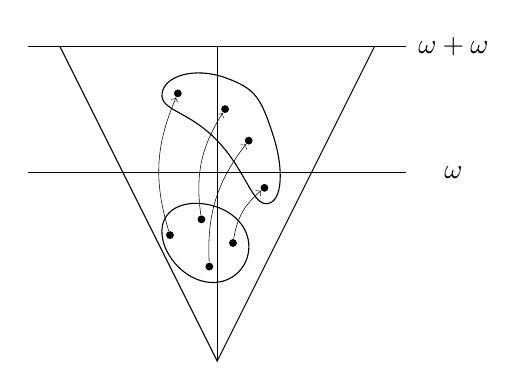
\begin{tikzpicture}[scale=2]
    \draw (1,2) -- (0,0) -- (-1,2);
    \draw (-1.2,2) -- (1.2,2);
    \draw [very thin] (-1.2,1.2) -- (1.2,1.2);
    \draw [very thin] (0,0) -- (0,2);
    \node at (1.5,2) {$\omega+\omega$};
    \node at (1.5,1.2) {$\omega$};
    \node [dot] (x1) at (-0.3,0.8) {};
    \node [dot] (x2) at (-0.05,0.6) {};
    \node [dot] (x3) at (0.1,0.75) {};
    \node [dot] (x4) at (-0.1,0.9) {};
    \draw plot [smooth cycle, tension=1] coordinates {(-0.35,0.8) (-0.05,0.5) (0.2,0.75) (-0.1,1)};
    \node [dot] (y1) at (-0.25,1.7) {};
    \node [dot] (y2) at (0.2,1.4) {};
    \node [dot] (y3) at (0.3,1.1) {};
    \node [dot] (y4) at (0.05,1.6) {};
    \draw [->, very thin] (x1) to[bend left=20] (y1);
    \draw [->, very thin] (x2) to[bend left=20] (y2);
    \draw [->, very thin] (x3) to[bend left=20] (y3);
    \draw [->, very thin] (x4) to[bend left=20] (y4);
    \draw plot [smooth cycle, tension=1] coordinates {(-0.35,1.7) (0.05,1.8) (0.35,1.45) (0.32,1.0) (0,1.4)};
  \end{tikzpicture}
\end{center}
\begin{idea}
  Take $x = \omega$, and
  \begin{equation*}
    F:
    \begin{cases}
      n \mapsto \omega + n \\
      y \mapsto 0 & \text{if } y \not\in \omega
    \end{cases}
  \end{equation*}
  Note $\omega+n$ is definable (in \hyperlink{def:axioms}{\textsf{Z}}): it is the unique \hyperlink{def:ordinal}{ordinal} which contains $\omega$ and $n-1$ elements above $\omega$.
\end{idea}
Let $Y \coloneqq \{F(n) \mid n \in \omega\}$. Then $\hyperlink{def:vk}{Y \subseteq V_{\omega+\omega}}$, but $Y \notin V_{\omega+\omega}$: it is not bounded in $V_{\omega+\omega}$.
\begin{center}
  \begin{tikzpicture}[scale=2]
    \draw (1,2) -- (0,0) -- (-1,2);
    \draw (-1.2,2) -- (1.2,2);
    \draw [very thin] (-1.2,1) -- (1.2,1);
    \draw [very thin] (0,0) -- (0,2);
    \node at (1.5,2) {$\omega+\omega$};
    \node at (1.5,1) {$\omega$};
    \draw [opacity=0.5, line width=3pt, line cap=round, bred] (0,0.75pt) -- (0, 1cm-0.75pt);
    \draw [opacity=0.5, line width=3pt, line cap=round, bblue] (0, 1cm+0.75pt) -- (0, 2cm-0.75pt);
    \foreach \x in {1,3,...,9}{
      \draw [->, bblue, thick] (0.5pt,\x*0.1) to[bend right=60] (0.5pt,1+\x*0.1);
    }
  \end{tikzpicture}
\end{center}
This example shows concretely that
\begin{equation*}
  V_{\omega + \omega} \models \neg \textsf{Repl.}
\end{equation*}

Similarly, if $\alpha$ is any \hyperlink{def:ordinal}{ordinal} such that there is a definable function $f: \omega \to \alpha$ such that the range of $f$ is unbounded in $\alpha$, then $V_\alpha \models \neg\textsf{Repl}$.
Even more generally, if $\beta < \alpha$ and a definable function $f: \beta \to \alpha$ with unbounded image, then $V_\alpha \models \neg\textsf{Repl}$.

\begin{defi}\hypertarget{def:reg}
  We call a cardinal $\kappa$ \named{regular} if there is no partition
  \begin{equation*}
    \kappa = \bigcup_{i \in I} A_i
  \end{equation*}
  such that $|I|, |A_i| < \kappa$ for all $i \in I$.
  Equivalently, for every $\alpha < \kappa$, there is no unbounded function $f: \alpha \to \kappa$.
\end{defi}

We know, e.g.\ that $\aleph_1$ is \hyperlink{def:reg}{regular}. Moreover, for any $\alpha$, $\aleph_{\alpha+1}$ is \hyperlink{def:reg}{regular}.
So our next candidate is $\alpha = \aleph_1$.

\begin{center}
  \begin{tikzpicture}[scale=2]
    \draw (1,2) -- (0,0) -- (-1,2);
    \draw (-1.2,2) -- (1.2,2);
    \draw [very thin] (-0.7,0.5) -- (0.7,0.5);
    \draw [very thin] (0,0) -- (0,2);
    \node at (1.5,2) {$\omega_1$};
    \node at (0.9,0.5) {$\omega$};
    \node [circle, fill=black, inner sep=1pt] at (-0.2, 0.6) {};
  \end{tikzpicture}
\end{center}
Note $\mathcal{P}(\omega) \in \hyperlink{def:vk}{V_{\omega+2}} \subseteq V_{\omega+1}$.
Clearly, there is a surjection
\begin{equation*}
  s: \mathcal{P}(\omega) \to \omega_1.
\end{equation*}
so the range of $s$ is unbounded in $\omega_1$.
Thus: $V_{\omega_1} \models \neg\textsf{Repl}$.

\begin{defi}\hypertarget{def:inacc}
  A cardinal $\alpha$ is called \named{inaccessible} if
  \begin{enumerate}[(a)]
    \item $\kappa$ is \hyperlink{def:reg}{regular}
    \item $\forall \lambda < \kappa$, $|\mathcal{P}(\lambda)| < \kappa$ (\named{strong limit}).
  \end{enumerate}
\end{defi}
That is, just take the two problems we had, negate them and make a definition.

\begin{remark}
  We know every successor cardinal is \hyperlink{def:reg}{regular}, and our simple examples of limit cardinals are all not regular: they were defined as unions.
  So, we can ask: `Are there regular limit cardinals?'
  (Such cardinals are sometimes called \named{weakly inaccessible}\index{inaccessible!weakly}).
  A partial answer: Under the Generalized Continuum Hypothesis ($\forall \kappa\ 2^\kappa = k^+$), we have:
  \begin{equation*}
    \kappa \text{ is inaccessible } \iff \kappa \text{ is a regular limit cardinal}.
  \end{equation*}
\end{remark}

Now, let's assume that $\kappa > \aleph_0$ is inaccessible.
\begin{lemma}
  \begin{equation*}
    \forall \lambda < \kappa \quad |\hyperlink{def:vk}{V_\lambda}| < \kappa.
  \end{equation*}
\end{lemma}
\begin{proof}
  Clearly $|\hyperlink{def:vk}{V_\omega}| = \aleph_0$, so $|V_\omega| < \kappa$.
  Proceed by induction. Suppose $|V_\lambda| < \kappa$. Then $V_{\lambda+1} = \mathcal{P}(V_\lambda)$.
  \begin{equation*}
  |V_{\lambda+1}| = |\mathcal{P}(V_\lambda)| < \kappa
  \end{equation*}
  by (b).
  Now let $\lambda < \kappa$ be a limit ordinal.
  Then
  \begin{equation*}
    V_\lambda = \bigcup_{\alpha < \lambda} V_\alpha.
  \end{equation*}
  Suppose for contradiction that $|V_\lambda| = \kappa$. But $|V_\alpha| < \kappa$ for all $\alpha < \kappa$, so you can write $\kappa$ as a union of $\lambda$ many things of smaller cardinality.
  This contradicts \hyperlink{def:reg}{regularity}.
\end{proof}

\begin{thm}
  If $\kappa$ is \hyperlink{def:inacc}{inaccessible}, then $\hyperlink{def:vk}{V_\kappa} \models \textsf{Repl}.$
\end{thm}
\begin{proof}
  Take any $F: V_\kappa \to V_\kappa$ and any $x \in V_\kappa = \bigcup_{\alpha < \kappa} V_\alpha$.
  Thus, find $\alpha \in \kappa$ such that $x \in V_\alpha$.
  Since $V_\alpha$ is transitive, $x \subseteq V_\alpha$.
  So $|x| \leq |V_\alpha| < \kappa$ (by the lemma).

  Now consider $X \coloneqq \{F(y) \mid y \in x\}$.
  For each $y \in x$, consider $\rho(F(y)) \coloneqq$ least $\alpha$ such that $F(y) \in V_{\alpha+1}\setminus V_\alpha$.
  By assumption, $\rho(F(y)) < \kappa$.
  Consider $\{\rho(F(y)) | y \in x\} \eqqcolon R$, then $|R| \leq |x| < \kappa$.
  By regularity, $\alpha \coloneqq \bigcup R < \kappa$.
  But $\forall y \in x \ F(y) \in V_{\alpha+1}$.
  So $X \subseteq V_{\alpha+1}$, $X \in V_{\alpha+2}$. This proves Replacement.
\end{proof}

Note we didn't even use that $F$ was definable: we showed a statement stronger than Replacement.
As a consequence, we get that the existence of inaccessible cardinals cannot be proved in \textsf{ZFC}.

\newlec Write \textsf{IC} for the axiom `there is an \hyperlink{def:inacc}{inaccessible} cardinal'.
If $\kappa$ is inaccessible, then $V_\kappa \models \textsf{ZFC}$.
$V_\kappa$ is a transitive model of \textsf{ZFC}, so,
\begin{equation*}
  \textsf{ZFC} + \textsf{IC} \vdash \underbrace{\text{`there is a transitive set that is a model of }\textsf{ZFC}\text{'}}_{\beta}
\end{equation*}
Recall that $\textsf{ZFC} + \cons{\textsf{ZFC}} \nvdash \beta$, so $\textsf{ZFC} + \cons{\textsf{ZFC}} \nvdash \textsf{IC}$.

\subsubsection{Model-theoretic reminders}
\begin{enumerate}
  \item L\"owenheim-Skolem theorem:
    If $S$ is any structure in some countable first-order language $\mathcal{L}$ and $X \subseteq S$ is any subset, then there is a \textbf{Skolem hull} of $X$ in $S$,
    $X \subseteq \mathcal{H}^S(X) \subseteq S$ such that
    \begin{enumerate}
      \item $\mathcal{H}^S(X) \preccurlyeq S$ Recall $\preccurlyeq$ means elementary substructure, meaning that
        \begin{equation*}\forall \varphi \; \forall h_1, \dotsc, h_n \in \mathcal{H}^S(X), \quad \mathcal{H}^S(X) \models \varphi(h_1, \dotsc, h_n) \iff S \models \varphi(h_1, \dotsc, h_n)\end{equation*}
        \item
          $|\mathcal{H}^S(X)| \leq \max(\aleph_0, |X|)$
    \end{enumerate}

    \emph{Proof sketch}. The key ingredient for this theorem is the Tarski-Vaught criterion, which says that for $Z \subseteq S$, we have $Z \preccurlyeq S$ iff for every $\varphi$ and all $z_1, \dotsc, z_n$,
    \begin{equation*}
      S \models \exists x\; \varphi(x, z_1, \dotsc, z_n) \implies Z \models \exists x\; \varphi(x, z_1, \dotsc, z_n).
    \end{equation*}
    Observe there are $\max(\aleph_0, |X|)$ many possible $\varphi(x, z_1, \dotsc, z_n)$, so for each formula which we need to satisfy, take a witness in $S$ and add it into $X$.
    But this introduces new $z_i$, so we need to add more witnesses, so repeat this process and take a union. Specifically,
    \begin{align*}
      Z_0 &\coloneqq X \\
      Z_1 &\coloneqq Z_0 \cup \text{the witnesses for all tuples $\varphi, z_1, \dotsc, z_n$ where $z_1, \dotsc, z_n \in Z_0$} \\
      Z_{n+1} &\coloneqq Z_n \cup \text{the witnesses for all tuples $\varphi, z_1, \dotsc, z_n$ where $z_1, \dotsc, z_n \in Z_n$} \\
      Z &\coloneqq \bigcup_{n \in \mathbb{N}} Z_n.
    \end{align*}
    $Z$ is the required model. \qedhere

    Now, work in \textsf{ZFC} + \textsf{IC}. Suppose $(M, \in) \models \textsf{ZFC} + \textsf{IC}$, which contains $V_\kappa \models \textsf{ZFC}$ ($V_\kappa \subseteq M$).
    Apply L\"owenheim-Skolem to $V_\kappa$ with $X \coloneqq \emptyset$. Then
    \begin{equation*}
      H \coloneqq \mathcal{H}^{V_\kappa}(\emptyset) \preccurlyeq V_\kappa
    \end{equation*}
    and $\mathcal{H}^{V_\kappa}(\emptyset)$ has cardinality $\leq \aleph_0$, and $H \models \textsf{ZFC}$.

    There is a formula $\varphi$ such that $\varphi(x)$ iff $x$ is the least uncountable cardinal.
    We have $V_\kappa \models \exists x \varphi(x)$, but the only element that satisfies $\varphi$ in $V_\kappa$ is $\aleph_1$.
    So in the Skolem hull construction,
    \begin{equation*}
      \aleph_1 \in Z_1 \subseteq H
    \end{equation*}
    This implies $H$ can't be transitive, since $\aleph_1$ has uncountably many elements, but $H$ has only countably many.
  \item Mostowki Collapse Theorem:
    If $X$ is any set and $R \subseteq X \times X$ such that $R$ is well-founded and extensional, then there is a transitive set $T$ such that $(T, \in) \cong (X,R)$.

    Consider $(H,\in) \models \textsf{ZFC}$. Since $(H,\in) \models \textsf{ZFC}$, $\in$ is extensional on $H$.
    Since $\in$ (in $M$) is well-founded, $\in$ is well-founded on $H$.
    So, let $T$ be the Mostowski collapse of $H$: $T$ is transitive and
    \begin{equation*}
      (T,\in) \cong (H,\in).
    \end{equation*}
    But this is an isomorphism, so $(T,\in) \models \textsf{ZFC}$. It is a bijection also, so $|T| = |H| \leq \aleph_0$.

    Together: there is a countable transitive model of \textsf{ZFC}.
\end{enumerate}

Notice that
\begin{align*}
  \varphi(x) &\coloneqq \text{`}x \text{ is countable'} \\
             &= \exists f \; (f: x \to \mathbb{N}, f \text{ is injective})
\end{align*}
is $\Sigma_1^{\textsf{ZFC}}$, so is upwards absolute.
But this formula is not downwards absolute: If $\alpha \in \textrm{Ord}$, $\alpha \in T$ then $V_\kappa \models \alpha$ is countable. But since $(T,\in) \models \textsf{ZFC}$, there is some $\alpha \in T$ such that $(T,\in) \models \alpha$ is uncountable, so $V_\kappa$ and $T$ disagree about the truth value of $\varphi(\alpha)$.

Consider now
\begin{align*}
  \psi(x) &\coloneqq  \text{`}x \text{ is a cardinal'} \\
  &= \forall \alpha \ (\alpha < x \rightarrow \text{there is no injection from $x$ to $\alpha$}).
\end{align*}
This is $\Pi_1^{\textsf{ZFC}}$. In $(T,\in)$, take $\alpha$ least such that $(T,\in) \models \neq\varphi(\alpha)$.
Then $(T,\in) \models \alpha$ is a cardinal. Clearly, $V_\kappa \models \alpha$ is not a cardinal.

Note that if  $\lambda$ is an uncountable cardinal in $V_\kappa$, then $\lambda \notin T$, so the downwards absoluteness of $\psi$ is not very interesting.

Instead of building $\mathcal{H}^{V_\kappa}(\emptyset)$, build $H^* \coloneqq \mathcal{H}^{V_\kappa}(\omega_1 + 1)$.
Clearly $\omega_1 \in H$ and $\omega_1 \subseteq H$, so $\omega_1 \subseteq T^*$ and $\omega_1 \in T^*$. We have $|H^*| = \aleph_1$.
Now we have $V_\kappa \models \omega_1 \text{ is a cardinal}$, so by downwards absoluteness of $\psi$, so $T^* \models \omega_1$ is a cardinal.

% Let $\kappa$ be a cardinal. We say $X$ is hereditarily smaller than $\kappa$ if $\abs{\tcl(X)} < \kappa$.
% Let $H_\kappa \coloneqq \{X \mid X \text{ is hereditarily smaller than } \kappa\}$.
% Obviously transitive.
\printindex
\end{document}
